%!TEX root = Lefley - Mesh to voxel transformations for optimised physics-based interactions.tex
\appendix

\chapter{Expanded Tables}

\begin{figure}[h!]
\rightline{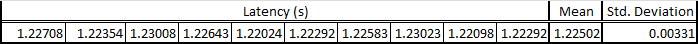
\includegraphics[scale=0.7]{../Logs/Instantiation.png}}
\caption{The time taken in seconds to instantiate 22 precomputed fragments over 10 runs.}
\label{fig:A.0.1}
\end{figure}

\begin{figure}[h!]
\rightline{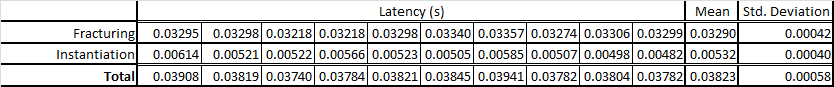
\includegraphics[scale=0.7]{../Logs/Fracture_Single_Sphere/Latency.png}}
\caption{The time in seconds when fracturing a sphere consisting of 760 triangles over 10 runs using Meshinator.}
\label{fig:A.1.1}
\end{figure}

\begin{figure}[h!]
\rightline{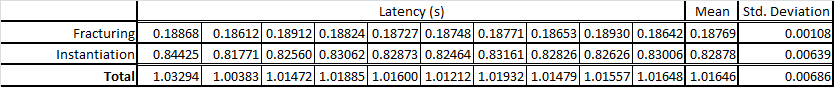
\includegraphics[scale=0.7]{../Logs/Fracture_Single_Bunny/Latency.png}}
\caption{The time in seconds when fracturing the Stanford Bunny, consisting of 69,666 triangles,s over 10 runs using Meshinator.}
\label{fig:A.2.1}
\end{figure}

\begin{figure}[h!]
\rightline{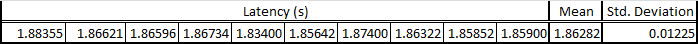
\includegraphics[scale=0.7]{../Logs/Fracture_Two_Bunny/Latency.png}}
\caption{The time taken in seconds to simultaneously fracture two Stanford Bunnies, each consisting of 69,666 triangles, over 10 runs using Meshinator.}
\label{fig:A.3.1}
\end{figure}

\begin{figure}[h!]
\rightline{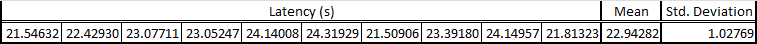
\includegraphics[scale=0.7]{../Logs/Voxel_Two_Bunny/Latency.png}}
\caption{The time taken in seconds to simultaneously fracture two Stanford Bunnies, each consisting of 69,666 triangles, over 10 runs using DVF.}
\label{fig:A.3}
\end{figure}

\begin{figure}[h!]
\rightline{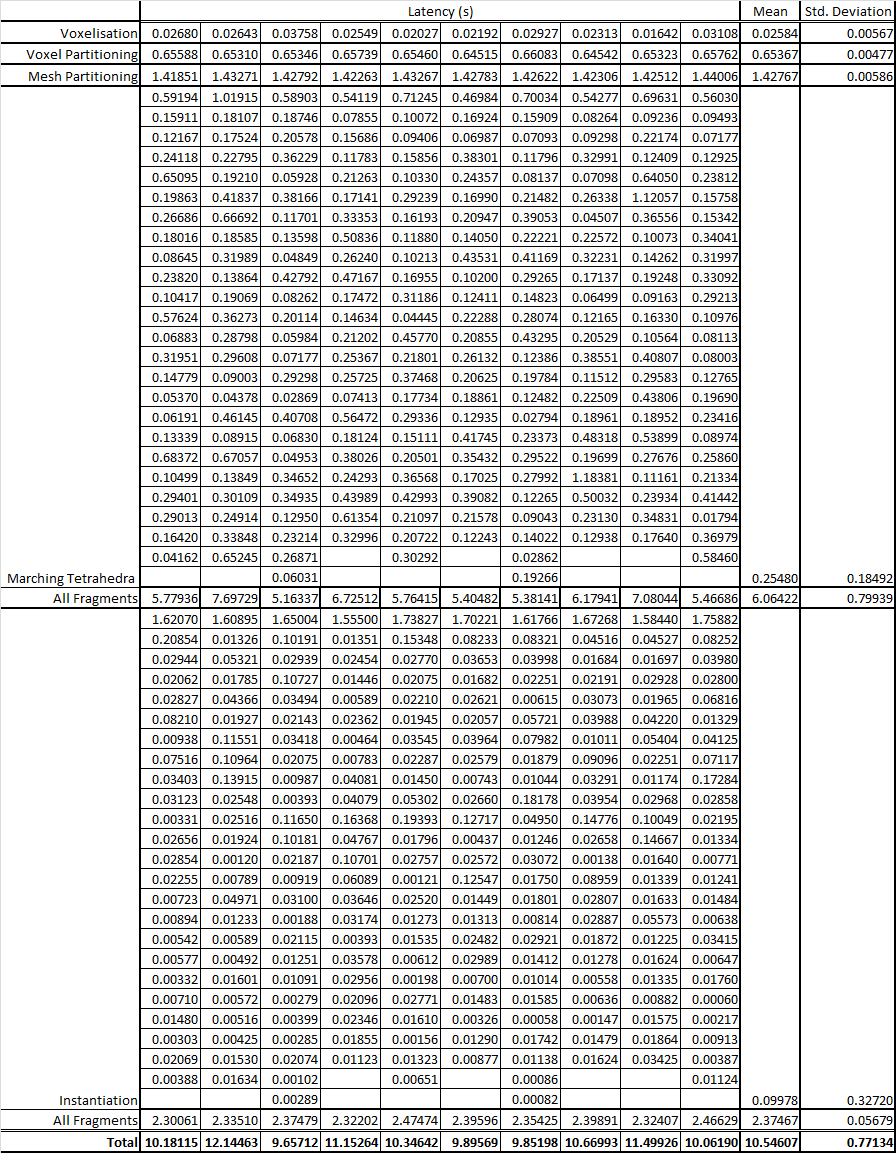
\includegraphics[scale=0.73]{../Logs/Voxel_Single_Bunny/Latency.png}}
\caption{The time in seconds by each pipeline stage when fracturing the Stanford Bunny, consisting of 69,666 triangles, over 10 runs using DVF. The number of generated fragments can vary slightly, resulting in the number of times the marching tetrahedra and instantiation phases are applied differing between runs.}
\label{fig:A.2}
\end{figure}

\begin{figure}[h!]
\rightline{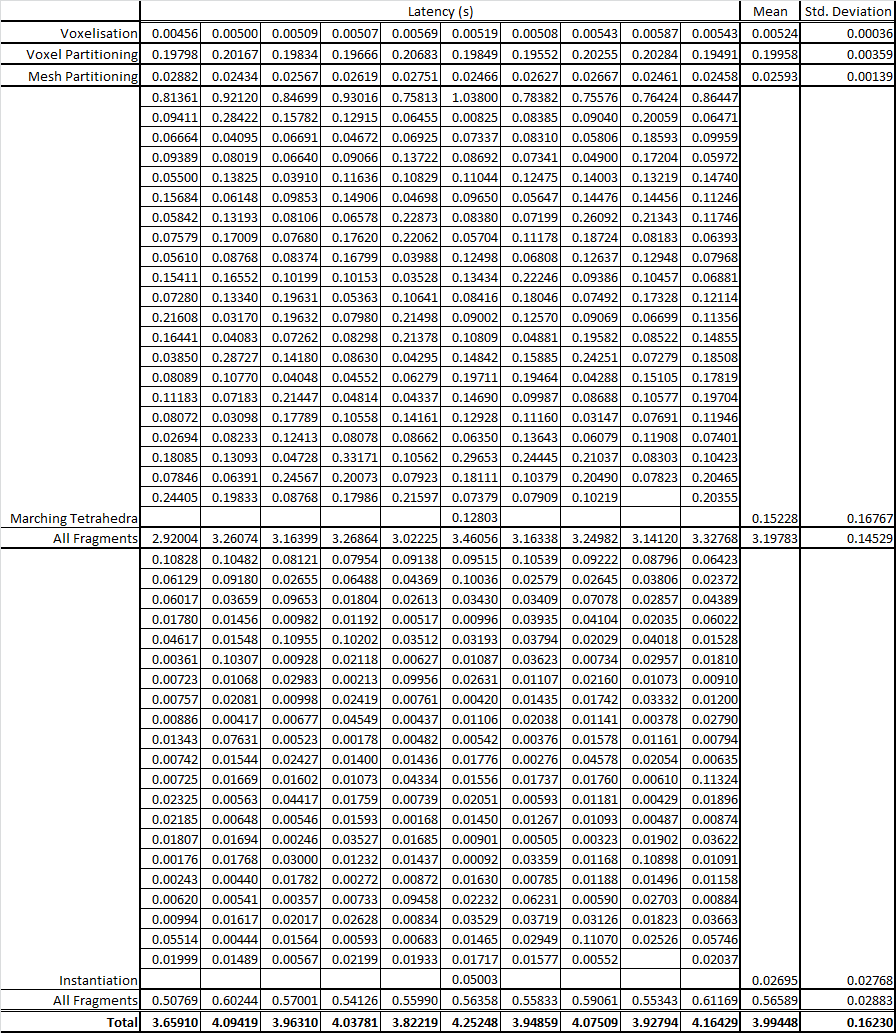
\includegraphics[scale=0.73]{../Logs/Voxel_Single_Sphere/Latency.png}}
\caption{The time in seconds by each pipeline stage when fracturing a sphere consisting of 760 triangles over 10 runs using DVF. The number of generated fragments can vary slightly, resulting in the number of times the marching tetrahedra and instantiation phases are applied differing between runs.}
\label{fig:A.1}
\end{figure}